\section{Text Attack}\label{sec:text-attack}
%**************************************************************
The only textual adversarial attack toolbox currently available are TextAttack \cite{journals/corr/abs-2005-05909} and OpenAttack \cite{journals/corr/abs-2009-09191}.
TextAttack is the earliest implemented tool and it is python framework to launch adversarial attacks, enable data augmentation and implement adversarial training for natural language process models. 
It can launch model-specific and evaluate the results, and improve robustness in the downstream and model generalization. 

TextAttack provides clean, readable implementations of 19 adversarial attacks from the literature.
All of these attacks are implemented as \emph{attack recipes} in TextAttack and can be benchmarked with just a single command.

%**************************************************************
\subsection{Framework structure}\label{subsec:framework-structure}

To unify adversarial attack methods into one
system, NLP attacks are decomposed into four components: a goal function, a set of constraints, a transformation, and a search method:
\begin{itemize}
    \item \textbf{Goal function}: determines whether the attack is successful in terms of the model outputs (eg. untargeted classification, targeted classification)
    \item \textbf{Constraints}: determine if a perturbation is valid with respect to the original input (eg. maximum word embedding distance, part-of-speech consistency)
    \item \textbf{Transformation}: generates a set of potential perturbations (eg. word swap, word insertion)
    \item \textbf{Search method}: successively queries the model and selects promising perturbations from a set of transformations (eg. greedy search, genetic algorithm)
\end{itemize}

This modular design enables us to easily assemble attacks from the literature while reusing components that are shared across attacks.

TextAttack's design also allows researchers to easily construct new attacks from combinations of novel and existing components.
Figure \ref{fig:2_4_textattack} shows the main components and features of TextAttack.

\begin{figure}[h]
    \centering
    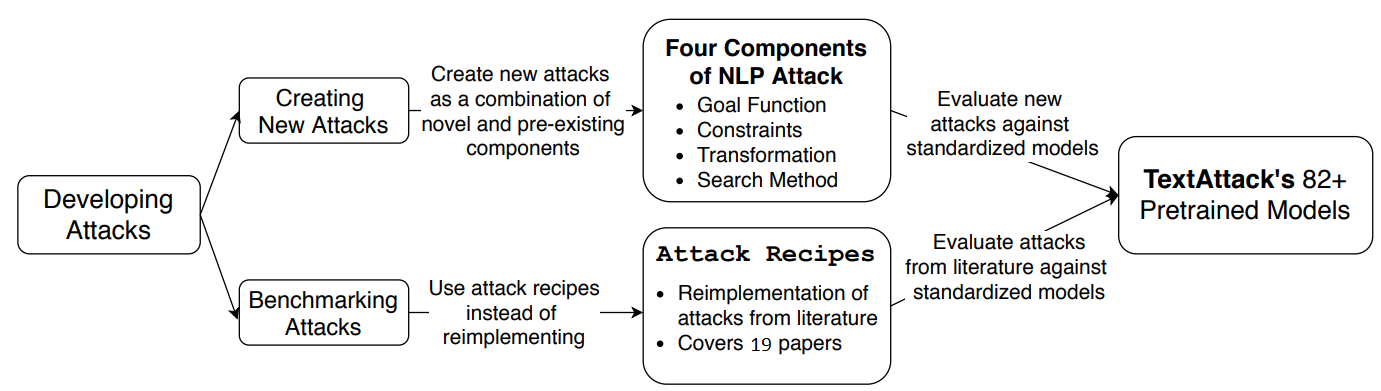
\includegraphics[width=0.9\linewidth]{images/2_4_textattack.png}
    \caption{Main features of of TextAttack}
    \label{fig:2_4_textattack}
\end{figure}

%**************************************************************
\subsection{HuggingFace integration}\label{subsec:huggingface-integration}

TextAttack is model-agnostic---meaning it
can run attacks on models implemented in any deep learning framework. Model objects must be able to take a string (or list of strings) and return an output that can be processed by the goal function.

TextAttack allows users to provide their own models and datasets. Moreover, it is directly integrated with HuggingFace\footnote{\url{https://huggingface.co}}'s transformers and NLP libraries. This allows users to test attacks on models and datasets publicly available on the platform. 

For benchmarck purpose, TextAttack
provides users with 82 pre-trained models, including word-level LSTM, word-level CNN, BERT, and other transformer based models pre-trained on various datasets provided by HuggingFace nlp. Since TextAttack is integrated with the nlp library, it can automatically load the test or validation data set for the corresponding pre-trained model \cite{journals/corr/abs-2005-05909}. 
